\documentclass{article}
\usepackage[utf8]{inputenc}
\usepackage[english, russian]{babel}
\usepackage{graphicx}
\usepackage[hcentering, bindingoffset = 10mm, right = 15 mm, left = 10 mm, top=20 mm, bottom = 20 mm]{geometry}
\DeclareGraphicsExtensions{.pdf,.png,.jpg}
\usepackage{tikz}
\usepackage{amsmath,amsfonts,amssymb,amsthm,mathtools}
\usepackage{multirow}
\usepackage{lipsum}
\usepackage{amsmath, amstext}
\usepackage{siunitx}
\usepackage{subcaption}
\usepackage{ upgreek }
\usepackage{wrapfig}
\usepackage{adjustbox}
\usepackage{enumerate, indentfirst, float}
\usepackage{capt-of, svg}
\usepackage{icomma}
\usepackage{amsmath}
\usepackage{ amssymb }
\usepackage{mathrsfs}
\usepackage{hyperref}
\usepackage{ gensymb }
\usepackage{fancyhdr}
\pagestyle{fancy}

\title{Московский Физико-Технический Институт}
\author{Кафедра общей физики \\ Лабораторная работа 5.5.5}
\begin{document}
	\maketitle
\thispagestyle{empty}
	\begin{center}
		\rule{\linewidth}{0.5mm} \\[0.4cm]
	{ \Huge\bfseries Изучение рассеяния медленных электронов на атомах (эффект Рамзауэра)\\ [0.4cm] }
		\rule{\linewidth}{0.5mm} \\[0.4cm]
	\end{center}	
\begin{minipage}{0.6\textwidth}
	\begin{flushleft} \large
		\emph{Авторы:}\\
		Рыбкина Елизавета\\
		Хомутов Андрей\\
	\end{flushleft}
\end{minipage}
\begin{center}
\end{center}
\fancyhead[C]{Лабораторная работа 5.5.5}
\newpage

\section*{Цель работы:}
Исследовать энергетическую зависимость вероятности рассеяния электронов атомами ксенона, определить энергии электронов, при которых наблюдается "просветление" ксенона, оценить размер его внешней электронной оболочки. 


\section*{Теоретическое описание}

\textit{Эффективное сечение реакции} --- это величина, характеризующая вероятность перехода системы двух сталкивающихся частиц в результате их рассеяния (упругого или неупругого) в определенное конечное состояние. Сечение $\sigma$ это отношение числа таких переходов $N$ в единицу времени к плотности потока $nv$ рассеиваемых частиц, падающих на мишень, т.е. к числу частиц, падающих в единицу времени на единичную площадку, перпендикулярно к их скорости.

\begin{equation}
\sigma = \frac{N}{nv}
\end{equation}

Эффект Рамзауэра нельзя объяснить с позиции классической теории. С квантовой же точки зрения картина рассеяния выглядит следующим образом: внутри атома потенциальная энергия падающего электрона отлична от нуля, скорость электрона меняется, становясь равной $v'$ в соответствии с законом сохранения энергии 

\[E = \frac{mv^2}{2} = \frac{mv'^2}{2}+U\]

а значит, изменяется и длина его волны де-Бройля. Таким образом, по отношению к электронной волне атом ведет себя как преломляющая среда с относительным показателем преломления
\begin{equation}
n = \frac{\lambda}{\lambda'} = \sqrt{1 - \frac{U}{E}}
\end{equation}

Решение задачи о рассеянии электрона на сферическом потенциале достаточно громоздко. Поэтому рассматривают более простое одномерное приближение: электрон рассеивается на потенциальной яме конечной глубины. После решения соответствующего уравнения Шрёдингера получается выражение для коэффициента прохождения:

\begin{equation}
D = \frac{16 k_1^2 k_2^2}{16k_1^2 k_2^2 + 4\left(k_1^2-k_2^2\right)^2\sin^2\left(k_2 l\right)}
\end{equation}
где $k_1^2 = \frac{2mE}{\hbar^2}, k_2^2 = \frac{2m(E + U_0)}{\hbar^2}$.

Как легко видно, это периодическое выражение с максимумами при 

\begin{equation}
k_2 l = \pi n = \sqrt{\frac{2m(E + U_0)}{\hbar^2}}l
\end{equation}

Это же условие можно получить, рассматривая интерференцию двух волн --- прошедшей через атом и отраженной от границ атомного потенциала. Тогда получаются следующие выражения для эффективного размера атома $l$:
\begin{equation}
2l = \frac{h}{\sqrt{2m(E_1 + U_0)}}
\end{equation}

\begin{equation}
2l = \frac{3}{2}\frac{h}{\sqrt{2m(E_2 + U_0)}}
\end{equation}

Где $E_1, E_2$ --- энергии, соответствующие максимуму и минимуму прохождения электронов соответственно. Исключая $U_0$ можно найти 

\begin{equation}
l = \frac{h\sqrt{5}}{\sqrt{32m(E_2 - E_1)}}
\end{equation}

\newpage

А исключая $l$ можно найти эффективную глубину потенциальной ямы атома:

\begin{equation}
U_0 = \frac{4}{5}E_2 - \frac{9}{5}E_1
\end{equation}

Так же можно вывести теоретически формулу, связывающую зависимость вероятности рассеяния электрона от его энергии:
\begin{equation}
w(V) = -\frac{1}{C} \ln \frac{I_a(V)}{I_0}
\end{equation}

С помощью неё, имея ВАХ тиратрона, можно построить график $w(V)$.

\section*{Схема установки}
Лампа-тиратрон ТГ301/1.3Б, заполненная инертным газом, расположена непосредственно на корпусе блока источников питания (БИП). Напряжение к электродам лампы подаются от источников питания, находящиеся в корпусе прибора. Регулировка напряжения и выбор режима работы установки производится при помощи ручек управления, выведенных на лицевую панель БИП.

\begin{figure}[H]
\begin{center}
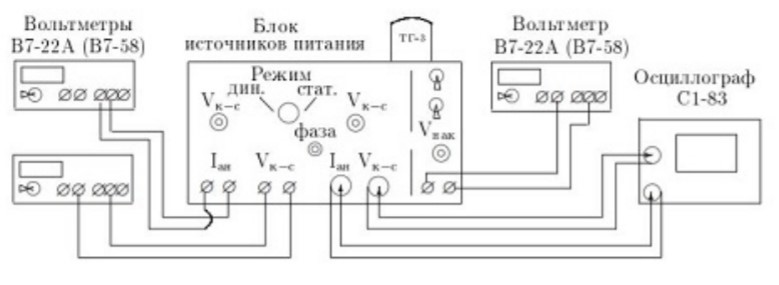
\includegraphics[width = 0.6\textwidth]{1}
\caption{Блок-схема экспериментальной установки}
\end{center}
\end{figure}

\section*{Ход работы и обработка результатов:}

\begin{enumerate}
	\item Подключили схему к сети переменного тока 220 В (частота 50 Гц).
	\item Вначале напряжения накала поставили на уровне 2-2.5 В, осцилограф работает в режиме внешней развертки.
	\item Плавно увеличивая подаваемое напряжение от генератора на тиратрон напряжение, наблюдали визуально вольт-амперную характеристику тиратрона, на которой отчетливо видны характеристические точки (максимумы и минимумы), связанные с проявлением эффекта Рамхауэра, и пробой газа.
	\item Поднесли к лампе постоянный магнит. Магнитное поле "обостряет" эффект Рамзауэра, так как оно отклоняет любой электрон, испытавший упругое столкновение. Убедилились, что это влияние зависит от ориентации магнита относительно оси тиратрона.
	
\end{enumerate}

\end{document}